\namedsubsection{FPGA}{Pasat}

An Field-Programmable Gate Array (FPGA) is a semiconductor device which is has a matrix of Configurable Logic Blocks (CLB) connected through programmable interconnects. One main advantage of the FPGA is that it can be preprogrammed after they are manufactured in order to fit desired functionalities and requirements. Interesting projects have also been realized with this processor on a FPGA, such as advanced real traffic light controller \cite{traffic_light}.

Typically, the FPGA differs from the conventional microcontroller; the microcontroller has the chip already designed. The programmer simply writes the software in C or C++, then it is compiled into a binary file that is loaded on the microcontroller. The program is stored in the flash memory until is is replaced or erased.

FPGAs are different in this sense. The circuit is completely designed by the programmer. The processor must be created and can be as simple as an and gate or can be our Cortex M0+. HDL is used to write the design, which is then synthesized into a bit file which configures the FPGA. One small problem with this is the fact that it stores the configuration in the RAM, so once the power is gone, the configuration is lost.

The board used for this project is the Xilinx Digilent Nexys4, which can be seen in figure \ref{fig:nexys4}. It is based on the Artix-7 which has a low power consumption and cost \cite{cortexm0onnexys4}. Implementations were also successful on low end FPGAs. This board was chosen because it is a large, high-capacity FPGA board that would be sufficient for our project. Another reason is the fact that is has several built in peripherals, such as accelerometer, which would be useful for the exercise detection. 

\begin{figure}
\centering
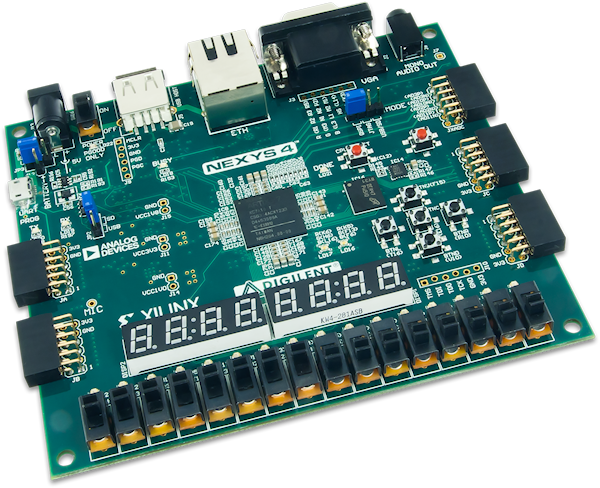
\includegraphics{figures/nexys4.PNG}
\caption{Xilinx Digilent Nexys4 \label{fig:nexys4}}
\end{figure}
